%% Inference-Aware Field Grading for Power Market Data Release
%% Target venue: SCI-indexed journal (energy informatics / information security)
%% Template: elsarticle (single column, preprint). Compile with pdfLaTeX + BibTeX on Overleaf.
\documentclass[preprint,12pt]{elsarticle}

\usepackage{amsmath,amssymb,amsthm}
\usepackage{graphicx}
\usepackage{booktabs}
\usepackage{multirow}
\usepackage{url}
\usepackage[hidelinks]{hyperref}

\graphicspath{{figures/}}

\newtheorem{definition}{Definition}
\newtheorem{theorem}{Theorem}
\newtheorem{proposition}{Proposition}
\newtheorem{corollary}{Corollary}
\newtheorem{remark}{Remark}

\newcommand{\Vy}{V_{y}}
\newcommand{\Mik}{M^{(K)}_{i \to y}}
\newcommand{\Rtwo}{R^{2}}
\DeclareMathOperator*{\argmax}{arg\,max}
\DeclareMathOperator*{\argmin}{arg\,min}

\journal{Elsevier}

\begin{document}

\begin{frontmatter}

\title{Inference-Aware Field Grading for Power Market Data Release:\\
Amortized Subset Inferability and Budgeted Marginal Risk}

\author{Haocun Du}
\address{(affiliation to be completed)}

\begin{abstract}
Power market operators publish large numbers of operational fields, and each field is
typically screened for disclosure risk on its own. We show that this practice is unsafe:
a field that looks harmless in isolation can become the decisive piece once an adversary
holds one or two other published fields. We formalize release auditing as the estimation
of \emph{set-level inferability} $\Vy(S)$, the out-of-sample $\Rtwo$ that the strongest
attacker in a fixed family can reach for a sensitive target $Y_y$ using only the published
field set $S$. To make the many subset queries of an audit affordable, we amortize them
with a random-mask shared representation combined with a subset-specific closed-form ridge
readout; against a shared output head this reduces the mean absolute error of $\Vy$ by
$3.2\times$ and $4.6\times$ on two real markets. On top of $\Vy$ we define the
\emph{budgeted marginal inference capability} $\Mik$, the largest inference gain that
field $i$ can add over any background of at most $K$ other candidate fields, and we
characterize it as a budget-constrained marginal contribution index on a conditional
evaluation function. We prove a truncated super-efficiency bound that yields a staged
release budget, show that $\Mik$ is exactly the minimal threshold-independent safety
margin, and prove that $\tau$-criticality is equivalent to membership in a minimal unsafe
set of size at most $K+1$. On PJM and CAISO data with 41 candidate fields and 12 sensitive
targets, exhaustive dedicated retraining shows that at $\tau=0.7$ and $K=2$, 35 of 41 (PJM)
and 38 of 41 (CAISO) fields are safe alone but critical once at most two background fields
are added. In a release audit over all size-three field sets, a single-field rule releases
19.1\% (PJM) and 56.4\% (CAISO) of the genuinely unsafe sets, whereas the staged budget
derived from our bound releases none while rejecting fewer than half of the safe sets.
We further show that $\Mik$, being a maximum statistic, is inflated under weak attackers,
and therefore report it together with a certified lower bound and a calibrated interval.
\end{abstract}

\begin{keyword}
data release auditing \sep inference risk \sep power market data \sep
feature importance \sep amortized inference \sep marginal contribution
\end{keyword}

\end{frontmatter}

%===============================================================================
\section{Introduction}
%===============================================================================

Independent system operators publish extensive operational data: fuel-mix generation,
load forecasts, ancillary-service requirements, locational marginal prices, and interchange
schedules. Such transparency is mandated in most markets, yet the same data can be used to
infer quantities the operator does not intend to disclose, for example total generation,
metered load, or procured reserve volumes. Deciding which fields may be released is
therefore a recurring operational problem.

Current practice screens fields one at a time. A candidate field is released if its
correlation with a sensitive target is low, or if a model trained on that field alone
predicts the target poorly. This paper starts from the observation that such screening is
not merely imprecise but systematically unsafe in a specific way: it is blind to
\emph{combination risk}. On the two markets we study, at a threshold of $\tau=0.7$ and a
background budget of $K=2$, \textbf{35 of 41 fields in PJM and 38 of 41 in CAISO are
individually safe but become critical once an adversary additionally holds at most two
other candidate fields}. A single-field release rule consequently releases 19.1\% (PJM) and
56.4\% (CAISO) of the field sets that a retrained attacker can actually exploit.

Making this quantitative requires answering two questions in sequence.

\paragraph{Q1: how inferable is an arbitrary field set?}
For a sensitive target $Y_y$ and a candidate published set $S$, we need the out-of-sample
inference capability $\Vy(S)$ that an adversary could reach using only $X_S$. The direct
route---retraining a dedicated attacker for every $S$---is exact but costly, and an audit
issues many such queries: ad-hoc checks on proposed releases, exhaustive low-order sweeps,
and searches for dangerous background combinations. We therefore ask whether a single
target-agnostic pre-learning stage can serve a large number of different subset queries.

\paragraph{Q2: how does set-level inferability become a field-level security quantity?}
$\Vy(S)$ alone does not grade fields. What a data owner needs is: \emph{given that the
adversary already holds some background information, how much can publishing field $i$
increase the inferability of $Y_y$?} We answer this with the budgeted marginal inference
capability $\Mik$, together with the background that attains it---a \emph{witness} that
makes the risk auditable rather than merely numerical.

\paragraph{Contributions.}
\begin{enumerate}
\item We formalize power-data release auditing as estimation of set-level inferability,
separating three objects that are routinely conflated: the population optimum $\Vy^{*}$,
the empirical capability $\Vy^{\mathrm{ret}}$ of a fixed attacker family, and the amortized
estimate $\Vy^{\mathrm{amo}}$ (Section~\ref{sec:problem}).

\item We show that the right level at which to amortize is the \emph{representation}, not
the value. A random-mask shared backbone whose features feed a subset-specific closed-form
ridge readout reduces $\Vy$ error by $3.2\times$ (PJM) and $4.6\times$ (CAISO) relative to
a shared output head, and cuts the rate of dangerously underestimated sets from 33.6\% and
28.7\% to 12.6\% and 3.8\% (Sections~\ref{sec:model} and \ref{sec:exp-a}).

\item We define $\Mik$ with an explicit public baseline $B$ and adversary budget $K$,
identify it as a budget-constrained marginal contribution index on the conditional
evaluation function $v_B$, and prove three properties that the unconstrained index does not
provide: a truncated super-efficiency bound that yields a staged release budget
(Theorem~\ref{thm:super}), an exact characterization of $\Mik$ as the minimal
threshold-independent safety margin (Theorem~\ref{thm:margin}), and the equivalence between
$\tau$-criticality and membership in a minimal unsafe set of size at most $K+1$
(Theorem~\ref{thm:mus}) (Section~\ref{sec:mk}).

\item On PJM and CAISO we compute exact $M^{(0..2)}$ for all 41 candidate fields and 12
targets by exhaustive dedicated retraining under a three-attacker family, quantify how much
single-field screening misses, and show that the staged budget is the only rule among six
that achieves zero dangerous release at a practical rejection rate
(Section~\ref{sec:exp-b}).

\item We document two failure modes of the point estimate and the corresponding remedy.
The amortized estimator underestimates $\Mik$ for some fields, and $\Mik$ is a maximum
statistic whose value is \emph{inflated} when the attacker is weak---by 5--12\% at $K=2$
under a tenth of the auxiliary labels. Reporting a certified lower bound together with a
calibrated upper bound removes both (Sections~\ref{sec:exp-a} and \ref{sec:exp-b}).
\end{enumerate}

\begin{figure}[t]
\centering
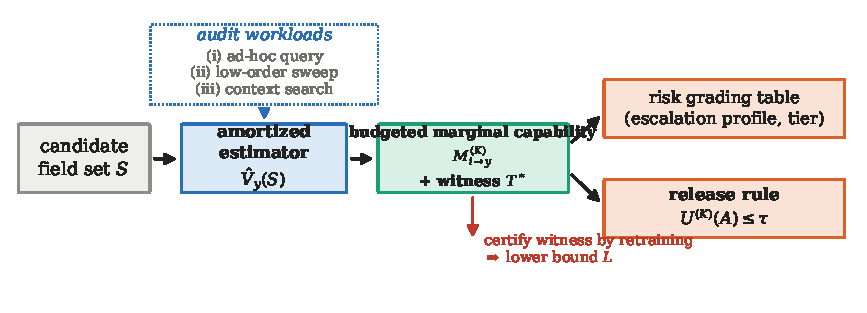
\includegraphics[width=\textwidth]{fig1_framework.pdf}
\caption{Audit pipeline. An arbitrary candidate field set $S$ is scored by the amortized
estimator $\hat V_y(S)$; sweeping low-order sets yields the budgeted marginal capability
$\Mik$ together with a witness background; the field-level table then drives risk grading
and a release rule. The three audit workloads that motivate amortization are marked.}
\label{fig:framework}
\end{figure}
\paragraph{What we do not claim.}
Random masking, closed-form ridge adaptation, maximum marginal contribution, and the notion
of a witness context all predate this work; Section~\ref{sec:related} attributes them.
We also do not claim that amortization is necessary at the scale studied here: with 41
fields, exhaustive parallel retraining completes the full $K\le 2$ audit in eleven minutes,
and we report this explicitly in Section~\ref{sec:exp-a}.

%===============================================================================
\section{Related Work}\label{sec:related}
%===============================================================================

\subsection{Privacy and inference leakage in power data}
Work on power-system privacy has concentrated on smart metering, where the concern is
recovering household activity from fine-grained consumption
traces~\cite{mcdaniel2009smartgrid,asghar2017smartmetering,giaconi2018smartmeter}.
Protection is usually achieved by perturbation or aggregation, with formal guarantees from
differential privacy~\cite{dwork2014dp} or syntactic models such as
$k$-anonymity~\cite{sweeney2002kanonymity}. These mechanisms answer a different question
from ours. They bound what can be learned about an \emph{individual record} after a release
mechanism is applied, whereas a market operator releasing aggregate operational series
needs to know which \emph{fields} may be published at all, given that an adversary can
train a supervised inference model on historical auxiliary labels. Our setting is closer to
attribute inference than to membership inference~\cite{shokri2017membership} or model
inversion~\cite{fredrikson2015inversion}, since the adversary attacks the published data
product rather than a deployed model.

\subsection{Feature importance and marginal contribution}
Shapley-based attribution~\cite{shapley1953value,lundberg2017shap,covert2020sage,
williamson2020spvim,covert2021explaining} distributes a fixed total among features. This is
the correct axiomatic answer for \emph{fair allocation}, but it is the wrong object for
disclosure risk: when two fields are near-duplicates, each receives roughly half the credit
even though either one alone enables the inference. Catav et al.~\cite{catav2021mci}
address exactly this dilution with the Marginal Contribution Index (MCI),
$I_\nu(f)=\max_{S}[\nu(S\cup\{f\})-\nu(S)]$, prove it is the unique function satisfying
marginal-contribution, elimination and minimalism axioms for monotone $\nu$, and establish
dummy, symmetry, super-efficiency, sub-additivity, a self-contribution lower bound, and
duplication invariance. They also introduce the maximizing set as a \emph{context}.
Our $\Mik$ inherits all of this. What we add is the security-relevant parameterization---a
public baseline $B$ and an explicit adversary budget $K$---and the theory that this
parameterization makes possible: the truncated bound and staged budget, the safety-margin
characterization, and the link to minimal unsafe sets. We use Shapley and
SAGE~\cite{covert2020sage} only as controls, and interaction
indices~\cite{grabisch1999interaction,sundararajan2020sti} only to explain why $M^{(1)}$
exceeds $M^{(0)}$. Model-reliance measures~\cite{breiman2001rf,fisher2019mcr} are likewise
controls: they describe what one fitted model uses, not what any attacker could achieve.

\subsection{Amortized prediction and fast adaptation}
Estimating $\Vy(S)$ for many $S$ is a set-conditioned prediction problem. Random feature
masking during training is standard in models that must handle arbitrary conditioning
patterns~\cite{ivanov2019vaeac,li2020acflow,you2020grape}, and amortization has been used
to avoid repeated per-instance optimization~\cite{cremer2018inference,amos2023amortized},
including amortized Shapley estimation~\cite{jethani2022fastshap,covert2023vitshapley}.
Closed-form ridge readouts on frozen features are the standard fast-adaptation mechanism in
meta-learning~\cite{bertinetto2019r2d2,lee2019metaoptnet}. Our contribution is not any of
these components but the finding, documented in Section~\ref{sec:exp-a}, that \emph{where}
one amortizes decides whether the estimate is usable: sharing the representation while
solving each subset's readout in closed form is markedly more faithful than sharing the
output head, and the difference is concentrated exactly on the high-marginal sets that
matter for security.

%===============================================================================
\section{Problem Formulation}\label{sec:problem}
%===============================================================================

\subsection{Threat model}
Two parties are involved.

The \textbf{auditor} is the data owner. It holds the complete historical record, including
the sensitive targets, and performs the audit offline before release.

The \textbf{adversary} obtains the published fields and is assumed to possess historical
auxiliary labels for the sensitive target, from which it trains an inference model. Risk is
therefore \emph{supervised inferability}, measured out of sample, not zero-shot inference.
Section~\ref{sec:exp-naux} studies how the conclusions change when the adversary's auxiliary
data is limited.

Let $G$ be the set of candidate publishable fields, $B \subseteq G$ the \emph{public
baseline} already released (default $B=\emptyset$), and $H = G \setminus B$ the fields under
audit. Let $Y_y$ denote a sensitive target. The adversary's \emph{background budget} $K$ is
the number of fields from $H$, beyond $B$, that it is assumed to already hold.

\subsection{Set-level inferability}
We distinguish three objects that are often conflated.

\begin{definition}[Population inferability]
$\Vy^{*}(S) = 1 - \inf_{f}\mathbb{E}[(Y_y - f(X_S))^{2}] / \mathrm{Var}(Y_y)$,
the infimum over all measurable $f$. It satisfies $\Vy^{*}(\emptyset)=0$,
$0 \le \Vy^{*} \le 1$, and is monotone in $S$, since additional fields may be ignored.
\end{definition}

\begin{definition}[Empirical inferability]
Given data split into $\mathrm{fit}$, $\mathrm{val}$ and $\mathrm{test}$, and an attacker
family $\mathcal{H}$, train each $h \in \mathcal{H}$ on $X_S$, select the attacker and its
training epoch on $\mathrm{val}$, and report test $\Rtwo$:
$\Vy^{\mathrm{ret}}(S) = \Rtwo_{\mathrm{test}}(\hat h_S)$,
$\hat h_S = \argmax_{h \in \mathcal{H},\,\mathrm{epoch}} \Rtwo_{\mathrm{val}}(h;S)$.
\end{definition}

Because of finite samples, optimization noise and selection noise, $\Vy^{\mathrm{ret}}$ is
not exactly monotone. An adversary holding $S$ may, however, train on any subset
$T \subseteq S$ and keep the best, so the operationally correct object is the
\emph{monotone closure}
\begin{equation}\label{eq:closure}
\bar V_y(S) = \Vy\big(\hat T_S\big), \qquad
\hat T_S = \argmax_{T \subseteq S} \Rtwo_{\mathrm{val}}(T),
\end{equation}
where the subset is chosen on validation data and the value is reported on test data.
This repairs finite-sample non-monotonicity without letting the test set influence any
selection. We write $\Vy$ for the closure throughout, and the closure applies equally to
the amortized estimate $\Vy^{\mathrm{amo}}$ defined in Section~\ref{sec:model}.
Since $\Mik$ only involves sets of size at most $K+1$, whose subsets are smaller still,
the closure does not destroy the locality of $\Mik$.

\subsection{Audit workloads}
The reason $\Vy$ must be cheap is not the abstract size of $2^{|G|}$ but three concrete
workloads: \emph{(i)} ad-hoc queries, where a proposed release set $S$ must be scored
immediately; \emph{(ii)} low-order exhaustive sweeps, where all sets up to a given size are
scored to build a field-level risk table; and \emph{(iii)} dangerous-context search, where
one looks for backgrounds that sharply amplify a field. Section~\ref{sec:exp-a} reports
where amortization does and does not pay off across these workloads.

\subsection{Data-use boundary}
For a given $S$, the closed-form readout uses only $Y_y^{\mathrm{train}}$ to obtain
$\beta_{y,S}$; the test prediction fixes this parameter, and $Y_y^{\mathrm{test}}$ enters
only the final $\Rtwo$. It never participates in backbone training, in solving $\beta$, in
selecting the ridge parameter, in checkpoint selection, or in witness search. We state this
explicitly because the auditor legitimately holds the sensitive labels, and the distinction
between using them for fitting and using them for reporting is what makes the reported
numbers out-of-sample.

%===============================================================================
\section{Amortized Subset-Universal Inference Model}\label{sec:model}
%===============================================================================

\subsection{Overview}
The model answers Q1: given a target $Y_y$ and an arbitrary $S \subseteq G$, produce an
estimate of $\Vy(S)$ without retraining a dedicated attacker. It has two stages. A
\emph{random-mask pre-learning} stage trains one backbone that must predict the targets from
randomly masked inputs, yielding a representation conditioned on which fields are visible.
A \emph{subset-specific adaptation} stage then solves, in closed form, a separate ridge
readout for each queried $(S, y)$ pair on top of frozen features.

\begin{figure}[t]
\centering
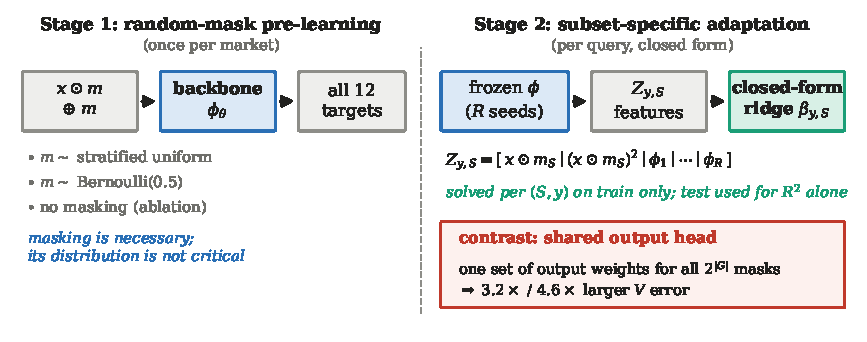
\includegraphics[width=\textwidth]{fig2_model.pdf}
\caption{Two stages of the estimator. Pre-learning trains one backbone under random masks
(left). At query time the backbone is frozen and only a subset-specific ridge readout is
solved in closed form (right); the contrast is with a shared output head, which reuses one
set of output weights for every conditioning pattern.}
\label{fig:model}
\end{figure}
\begin{remark}[Scope of ``universal'']
The model is universal \emph{over field subsets}, which is what the audit workloads require.
The backbone is shared across the 12 targets of a market; the readout is specific to both
the subset and the target. Our experimental plan initially specified a separate backbone per
target, but Section~\ref{sec:exp-a} shows that per-target backbones are uniformly worse and
twelve times more expensive to pre-train, so the shared backbone is the main configuration
and the per-target variant is reported as an ablation. Note that this concerns the
\emph{estimator}; the attacker family used to define ground truth does include single-target
networks, because there the goal is to be as strong as possible, not to amortize.
\end{remark}

\subsection{Random-mask pre-learning}
Let $m \in \{0,1\}^{|G|}$ be a visibility mask. The backbone
$\phi_\theta(x \odot m, m)$ is a multilayer perceptron taking the masked input concatenated
with the mask itself, trained to predict all sensitive targets under masks drawn from a
sampling distribution. Concatenating $m$ matters: without it, a zeroed field is
indistinguishable from a field whose standardized value happens to be zero. We take
$\phi$ to be the activation of the last hidden layer, a 256-dimensional vector.

The mask distribution is a design choice, and we report it as such. Section~\ref{sec:exp-a}
compares a stratified uniform sampler, a Bernoulli$(0.5)$ sampler and no masking at all;
the first two are nearly indistinguishable while removing masking degrades the estimate.
The honest summary is that random masking is necessary but its precise distribution is not
critical, and we make no claim of a novel sampling scheme.

\subsection{Subset-specific closed-form readout}
For a query $(S,y)$ with mask $m_S$, form the feature block
\begin{equation}
Z_{y,S} = \big[\; x \odot m_S \;\big|\; (x \odot m_S)^{2} \;\big|\;
\phi_{\theta_1}(x,m_S) \;\big|\; \cdots \;\big|\; \phi_{\theta_R}(x,m_S) \;\big],
\end{equation}
concatenating the masked raw inputs, their squares, and the frozen features of $R$
independently seeded backbones ($R=3$ in the main configuration). The readout is ridge
regression solved in closed form on the training split,
\begin{equation}\label{eq:ridge}
\beta_{y,S} = \big(Z^{\top}_{\mathrm{fit}} Z_{\mathrm{fit}} + \lambda I\big)^{-1}
Z^{\top}_{\mathrm{fit}} Y^{\mathrm{fit}}_{y},
\end{equation}
with $\lambda$ chosen on a fit/val partition \emph{inside} the training split. The estimate
is the test $\Rtwo$ of $Z^{\mathrm{test}}_{y,S}\beta_{y,S}$, after which the monotone
closure \eqref{eq:closure} is applied. Solving \eqref{eq:ridge} costs one small linear
system, so a query is milliseconds rather than the tens of seconds a dedicated retraining
requires.

\subsection{Why not a shared output head}
The alternative amortization---let one network map $(x \odot m, m)$ directly to the
predicted target, and read $\Vy(S)$ off its output---is strictly cheaper at query time and
is what most masked-input models do. It is also substantially less faithful, and the gap is
not uniform: it concentrates on sets with large marginal gains, which are precisely the ones
that decide a release. Section~\ref{sec:exp-a} quantifies this. The mechanism is that a
single set of output weights must serve all $2^{|G|}$ conditioning patterns, so the head
interpolates across subsets; solving each subset's readout separately removes this
interference while keeping the expensive representation shared.

\subsection{Error propagation to $\Mik$}
Let $\tilde V$ be the closed estimate and $\tilde\Delta$ the induced marginals. Since the
maximum is $1$-Lipschitz in the supremum norm and a marginal is a difference of two values,
\begin{equation}\label{eq:prop}
\big|\tilde M^{(K)}_{i\to y} - \Mik\big|
\;\le\; \max_{|T| \le K}\big|\tilde\Delta_i(T) - \Delta_i(T)\big|
\;\le\; 2 \max_{|S| \le K+1}\big|\tilde V(B \cup S) - V(B \cup S)\big| .
\end{equation}
The practical consequence is that the quantity to control is the \emph{marginal} error, not
the value error: an estimator with a small bias in $V$ can still misrank fields if its error
is correlated across the two sets forming a marginal. We report marginal error explicitly.

%===============================================================================
\section{Budgeted Marginal Inference Capability}\label{sec:mk}
%===============================================================================

\subsection{Definition}
\begin{definition}[Budgeted marginal inference capability]\label{def:mk}
For target $y$, public baseline $B$, candidate set $H=G\setminus B$ and budget $K$,
\begin{equation}
\Mik \;=\; \max_{T \subseteq H \setminus \{i\},\, |T| \le K}
\Big[\, \Vy(B \cup T \cup \{i\}) - \Vy(B \cup T) \,\Big].
\end{equation}
Any $T^{*}$ attaining the maximum is a \emph{witness background}.
\end{definition}

Two derived quantities are used for interpretation only:
the single-field capability $a^{B}_{i} = M^{(0)}_{i \to y} = \Vy(B\cup\{i\}) - \Vy(B)$,
and the second-order interaction
$I^{B}_{ij} = \Vy(B\cup\{i,j\}) - \Vy(B\cup\{i\}) - \Vy(B\cup\{j\}) + \Vy(B)$.

\subsection{Relation to the marginal contribution index}
\begin{proposition}\label{prop:mci}
Let $v_B(T) := \Vy(B \cup T) - \Vy(B)$ for $T \subseteq H$. Then
\emph{(a)} $v_B$ is monotone, non-negative and satisfies $v_B(\emptyset)=0$, hence meets all
assumptions Catav et al.~\cite{catav2021mci} impose on an evaluation function;
\emph{(b)} $\Mik = \max_{|T|\le K}[v_B(T\cup\{i\}) - v_B(T)]$, i.e.\ $\Mik$ is the
\emph{budget-constrained} MCI of $v_B$;
\emph{(c)} for $K \ge |H|-1$, $\Mik$ equals the unconstrained MCI of $v_B$, and for
$B=\emptyset$ the original MCI of $\Vy$.
\end{proposition}
\begin{proof}
(a) $\Vy$ is monotone and $B\cup T \subseteq B\cup T'$ whenever $T\subseteq T'$; also
$v_B(\emptyset)=\Vy(B)-\Vy(B)=0$. (b) Substituting the definition,
$\Vy(B\cup T\cup\{i\})-\Vy(B\cup T)=v_B(T\cup\{i\})-v_B(T)$. (c) The budget constraint
becomes vacuous, so the feasible set is all $T\subseteq H\setminus\{i\}$.
\end{proof}

By Proposition~\ref{prop:mci}, every property MCI enjoys for monotone $\nu$---dummy, symmetry,
sub-additivity, the self-contribution lower bound $\Mik \ge \Vy(B\cup\{i\})-\Vy(B)$,
duplication invariance, and the dilution argument against Shapley---transfers to $\Mik$
and is cited rather than claimed. What does not transfer is everything that depends on the
budget being finite, and that is where our theory lies. We state three results; proofs of
the remaining propositions are in \ref{app:proofs}.

\subsection{Truncated super-efficiency and the staged budget}
\begin{theorem}[Truncated super-efficiency]\label{thm:super}
For any $A \subseteq H$:
\begin{enumerate}
\item[(a)] if $|A| \le K+1$, then
$\Vy(B \cup A) - \Vy(B) \;\le\; \sum_{i \in A} \Mik$;
\item[(b)] define $U^{(K)}(\emptyset)=0$ and
$U^{(K)}(A) = \min_{j \in A}\big[\,U^{(K)}(A\setminus\{j\}) +
M^{(\min(|A|-1,\,K))}_{j \to y}\,\big]$.
If $|A| \le K+1$, then
$\Vy(B\cup A)-\Vy(B) \;\le\; U^{(K)}(A) \;\le\; \sum_{i\in A}\Mik$;
\item[(c)] if $M^{(K)}_{i\to y} = M^{(|A|-1)}_{i \to y}$ for all $i \in A$, then (a) and (b)
hold without the restriction $|A| \le K+1$.
\end{enumerate}
\end{theorem}
\begin{proof}
(a) Fix any order $i_1,\dots,i_m$ of $A$ with $m=|A|$ and let $A_t=\{i_1,\dots,i_t\}$.
Telescoping, $v_B(A)=\sum_{t=1}^{m}[v_B(A_t)-v_B(A_{t-1})]$. The $t$-th term is the
marginal of $i_t$ over a background of size $t-1 \le K$, hence at most
$M^{(K)}_{i_t \to y}$. Only $v_B(\emptyset)=0$ is used.
(b) Induct on $|A|$: $v_B(A)=v_B(A\setminus\{j\})+\Delta_j(B\cup A\setminus\{j\})
\le U^{(K)}(A\setminus\{j\}) + M^{(|A|-1)}_{j\to y}$, then minimize over $j$; the second
inequality follows from monotonicity of $M^{(k)}$ in $k$ (Proposition~\ref{prop:ladder}).
(c) Replace each bound in (a) by $M^{(|A|-1)} = M^{(K)}$.
\end{proof}

\begin{remark}
For $K \ge |H|-1$ part (a) reduces to the super-efficiency of~\cite{catav2021mci} on $v_B$.
It is not a corollary of it: since $\Mik \le \mathrm{MCI}$, the truncated inequality is
\emph{stronger}, and needs its own proof, although the telescoping technique is the same.
Parts (b) and (c) have no unconstrained counterpart. Part (b) is what we deploy as the
\emph{staged budget} release rule in Section~\ref{sec:exp-b}: it is tighter than the
additive budget of (a) because a set of size three need not charge every member at the
full budget $K$.
\end{remark}

\subsection{$\Mik$ as the minimal threshold-independent safety margin}
\begin{theorem}[Safety margin]\label{thm:margin}
Fix $i$, $y$, $B$ and $K$. Consider three notions of margin:
a \emph{uniform marginal bound} $m$ satisfying $\Delta_i(B\cup T)\le m$ for all $|T|\le K$;
a \emph{universal margin} $m$ satisfying
``for all $\tau$ and all $|T|\le K$: $\Vy(B\cup T)\le \tau-m \Rightarrow
\Vy(B\cup T\cup\{i\})\le\tau$'';
and, for a fixed $\tau$, $m_\tau=\inf\{m\ge 0:\ \forall |T|\le K,\
\Vy(B\cup T)\le\tau-m \Rightarrow \Vy(B\cup T\cup\{i\})\le\tau\}$. Then
\emph{(a)} $m$ is a uniform marginal bound $\iff$ $m$ is a universal margin $\iff$
$m \ge \Mik$, so $\Mik$ is the \emph{minimal universal margin};
\emph{(b)} $m_\tau \le \Mik$ for every $\tau$, and the inequality can be strict.
\end{theorem}
\begin{proof}
(a) The first equivalence is the definition of the maximum. Universal margin $\Rightarrow$
uniform bound: for any $T$ take $\tau=\Vy(B\cup T)+m$, giving $\Delta_i(B\cup T)\le m$.
Uniform bound $\Rightarrow$ universal margin: $\Vy(B\cup T\cup\{i\})=\Vy(B\cup T)+\Delta
\le (\tau-m)+m=\tau$. (b) $\Mik$ satisfies the fixed-$\tau$ condition, so
$m_\tau\le\Mik$. Strictness: with $B=\emptyset$, $K=1$, $\Vy(\{i\})=0.1$, $\Vy(\{j\})=0.5$,
$\Vy(\{i,j\})=0.9$, we get $M^{(1)}_{i}=0.4$, while at $\tau=0.95$ no admissible background
can be pushed above $\tau$ by adding $i$, so $m_\tau=0$.
\end{proof}

Theorem~\ref{thm:margin} is why $\Mik$ belongs in a grading table: it is a property of the
field that does not depend on the threshold eventually chosen. It also delimits the claim:
for one fixed $\tau$ the necessary margin may be strictly smaller, so using $\Mik$ as a
release budget at a fixed threshold is conservative. We therefore do not describe $\Mik$ as
``the minimal margin at a given $\tau$''.

\subsection{Criticality and minimal unsafe sets}
\begin{definition}
Under baseline $B$, a set $E\subseteq H$ is a \emph{$\tau$-minimal unsafe set} (MUS) if
$\Vy(B\cup E)>\tau$ while $\Vy(B\cup E')\le\tau$ for every $E'\subsetneq E$. A field $i$ is
\emph{$K$-background $\tau$-critical} if there exists $T$ with $|T|\le K$, $i\notin T$, such
that $\Vy(B\cup T)\le\tau<\Vy(B\cup T\cup\{i\})$.
\end{definition}

\begin{theorem}[Criticality $\iff$ small MUS]\label{thm:mus}
If $\Vy$ is monotone and $\Vy(B)\le\tau$, then $i$ is $K$-background $\tau$-critical if and
only if $i$ belongs to some MUS of size at most $K+1$.
\end{theorem}
\begin{proof}
($\Leftarrow$) Let $E \ni i$ be a MUS with $|E|\le K+1$ and take $T=E\setminus\{i\}$. By
minimality $\Vy(B\cup T)\le\tau$, and $\Vy(B\cup E)>\tau$.
($\Rightarrow$) Suppose $\Vy(B\cup T)\le\tau<\Vy(B\cup T\cup\{i\})$. Among the unsafe
subsets of $T\cup\{i\}$ choose one, $E$, minimal under inclusion; it is a MUS with
$|E|\le K+1$. If $i\notin E$ then $E\subseteq T$, and \emph{monotonicity} gives
$\Vy(B\cup T)\ge \Vy(B\cup E)>\tau$, a contradiction.
\end{proof}

Monotonicity is not decorative here. With $\Vy(\{1\})=0.8$, $\Vy(\{3\})=0.2$,
$\Vy(\{1,3\})=0.2$, $\Vy(\{1,2,3\})=0.9$ and $\tau=0.5$, field 2 crosses the threshold over
background $\{1,3\}$, yet every unsafe set containing field 2 also contains the unsafe
proper subset $\{1\}$, so no MUS contains it. This is one of the reasons the monotone
closure \eqref{eq:closure} is applied before any $\Mik$ is computed; on raw
$\Vy^{\mathrm{ret}}$ we observed a 0.2\% violation rate, which the closure removes.

\subsection{Closed form at $K=1$ and the role of interaction}
\begin{proposition}\label{prop:k1}
$M^{(0)}_{i\to y}=a^{B}_{i}$ and
$M^{(1)}_{i\to y}=a^{B}_{i}+\max\big(0,\ \max_{j \in H\setminus\{i\}} I^{B}_{ij}\big)$.
\end{proposition}
\begin{proof}
For $K=0$ the only background is $\emptyset$. For $K=1$ the background is $\emptyset$ or
some $\{j\}$, and $\Delta_i(B\cup\{j\})=\Vy(B\cup\{i,j\})-\Vy(B\cup\{j\})=a^{B}_{i}+I^{B}_{ij}$.
\end{proof}

Hence a field is escalated by a background partner \emph{exactly when} it is strictly
super-additive with that partner. This also shows why a naive synergy score is not the right
trigger: with $\mathrm{syn}_2(ij)=\Vy(\{i,j\})-\max(a_i,a_j)$ one has
$I_{ij}=\mathrm{syn}_2-\min(a_i,a_j)$, so $\mathrm{syn}_2>0$ does not imply escalation.

\subsection{From field risk to grading and release audit}
The audit deliverable per target is a table containing, for each field, the escalation
profile $(M^{(0)},M^{(1)},M^{(2)})$, the witness background attaining $M^{(2)}$, a risk tier,
and the $\tau$-critical flag. Because Theorem~\ref{thm:super}(b) bounds the inferability of a
whole proposed release set by a staged sum of field-level budgets, the same table also
supports a release rule: accept $A$ if $U^{(K)}(A)\le\tau$. Section~\ref{sec:exp-b} compares
this rule against correlation screening, single-field screening, an additive budget, and a
direct estimate of $\Vy(A)$.

%===============================================================================
\section{Experimental Setup}\label{sec:setup}
%===============================================================================

\subsection{Data and protocol}
We use one year of hourly operational data from two independent markets, PJM and CAISO
(Table~\ref{tab:data}). Preprocessing removes constant columns and rows with missing values,
then splits the records 70/30 into train and test with a fixed shuffle seed; 15\% of train
is held out as validation. Standardization uses train statistics only.

Fields that are exact or deterministic affine duplicates of another field are merged, since
they would otherwise inflate the field count without adding information; near-duplicates
($r<0.999$) are deliberately \emph{kept}, because such redundancy is precisely what the
method must handle. Visible copies of sensitive targets are removed. This leaves 41
candidate fields and 12 sensitive targets per market. The full field lists, the merge rules,
data fingerprints and the frozen protocol are provided as supplementary material; the
protocol was fixed before the reported experiments were run and was amended only three times,
each amendment recorded with its empirical justification.

\begin{table}[t]
\centering
\caption{Datasets and threat-model settings.}
\label{tab:data}
\small
\begin{tabular}{lll}
\toprule
& PJM & CAISO \\
\midrule
Complete records & 6{,}556 & 8{,}722 \\
Train / val / test & 4{,}589 (688 val) / 1{,}967 & 6{,}105 (916 val) / 2{,}617 \\
Candidate fields $|H|$ & 41 & 41 \\
Sensitive targets & 12 & 12 \\
Public baseline $B$ & $\emptyset$ (default); load forecasts (case study) & $\emptyset$ \\
Background budget $K$ & \multicolumn{2}{l}{$\{0,1,2\}$ in the main text, $K=3$ in \ref{app:k3}} \\
Threshold $\tau$ & \multicolumn{2}{l}{$\{0.5,0.7,0.9\}$, main text $0.7$} \\
\bottomrule
\end{tabular}
\end{table}

\subsection{Ground truth and attacker family}
Ground truth is exhaustive dedicated retraining. For every field set of size at most three
(18{,}000 sets per market) and every target, we train attackers using only that set. The
attacker family $\mathcal{H}$ contains a single-target network, a multi-target network, and
a histogram gradient-boosting regressor~\cite{ke2017lightgbm}; the family maximum is taken
after selecting attacker and epoch on validation, and the monotone closure
\eqref{eq:closure} is then applied.

Including all three matters. At set size three, the tree is selected for 55.2\% of
(set, target) pairs in PJM and 43.0\% in CAISO, and the single-target network for 35.3\% and
50.5\%. Using only the multi-target network---the natural choice if one reuses the estimator
architecture---understates ground truth by 0.0267 (PJM) and 0.0155 (CAISO) $\Rtwo$ at size
three, which is enough to flip $\tau$-critical decisions.

Dedicated retraining at this scale is feasible because the independent networks are trained
simultaneously as a batched tensor operation: masked inputs are zeroed, so the first-layer
weights of masked columns neither affect the output nor receive gradient, making the batched
computation functionally equivalent to training each network on its own columns. This reduces
the per-set cost from 21.8\,s (PJM, sequential) to 56.6\,ms at batch size 1024.

\subsection{Metrics}
For $\Vy$ we report mean absolute error, bias, Spearman correlation and the
\emph{dangerous-underestimation rate}, the fraction of (set, target) pairs whose estimate
falls below the truth by more than $0.05$. For $\Mik$ we report absolute error, Kendall
correlation of the field ranking, risk-tier agreement, witness recall
$P(L \ge M - 0.02)$ where $L$ is the certified lower bound, and $\tau$-critical
recall/precision. For release rules we report the \emph{dangerous release rate}, the fraction
of genuinely unsafe sets that the rule accepts, and the false rejection rate.

%===============================================================================
\section{Part A: Does Amortization Estimate $V$ and $M$ Reliably?}\label{sec:exp-a}
%===============================================================================

\subsection{RQ-A1/A2: fidelity and the level of amortization}
Table~\ref{tab:ablation} compares estimators against the three-attacker ground truth on all
sets of size at most three.

\begin{table}[t]
\centering
\caption{Estimator comparison against the official three-attacker ground truth, all sets of
size $\le 3$. ``Dangerous'' is the fraction of (set, target) pairs underestimated by more
than $0.05$. Best in each column in bold.}
\label{tab:ablation}
\small
\begin{tabular}{llrrrrr}
\toprule
Market & Estimator & $V$ MAE & $V$ bias & Dangerous & $M^{(2)}$ MAE & Witness recall \\
\midrule
\multirow{7}{*}{PJM}
 & raw ridge                  & 0.1230 & $-$0.1220 & 34.9\% & 0.1185 & 0.155 \\
 & raw $+\,x^2$ ridge         & 0.0898 & $-$0.0880 & 29.0\% & 0.0951 & 0.189 \\
 & random features            & 0.0441 & $-$0.0380 & 17.9\% & 0.0832 & 0.220 \\
 & \emph{shared output head}  & 0.0892 & $-$0.0875 & 33.6\% & 0.1179 & 0.152 \\
 & $\phi$ ridge               & 0.0319 & $-$0.0238 & 15.1\% & 0.0363 & 0.382 \\
 & per-target backbone        & 0.0403 & $-$0.0349 & 19.2\% & 0.0526 & 0.362 \\
 & \textbf{$\phi+x,x^2$ (3 seeds)} & \textbf{0.0276} & $-$\textbf{0.0180} & \textbf{12.6\%} & \textbf{0.0297} & 0.352 \\
\midrule
\multirow{7}{*}{CAISO}
 & raw ridge                  & 0.1041 & $-$0.1040 & 40.4\% & 0.0664 & 0.281 \\
 & raw $+\,x^2$ ridge         & 0.0676 & $-$0.0673 & 25.8\% & 0.0581 & 0.453 \\
 & random features            & 0.0204 & $-$0.0175 & 5.3\%  & 0.0340 & 0.474 \\
 & \emph{shared output head}  & 0.0705 & $-$0.0701 & 28.7\% & 0.0581 & 0.358 \\
 & $\phi$ ridge               & 0.0178 & $-$0.0143 & 4.6\%  & 0.0184 & 0.732 \\
 & per-target backbone        & 0.0230 & $-$0.0209 & 6.8\%  & 0.0230 & 0.587 \\
 & \textbf{$\phi+x,x^2$ (3 seeds)} & \textbf{0.0153} & $-$\textbf{0.0106} & \textbf{3.8\%} & \textbf{0.0141} & \textbf{0.742} \\
\bottomrule
\end{tabular}
\end{table}

\begin{figure}[t]
\centering
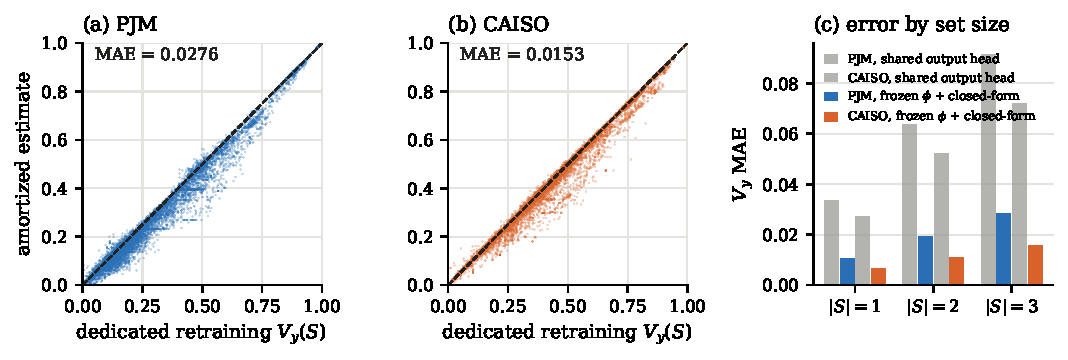
\includegraphics[width=\textwidth]{fig3_v_fidelity.pdf}
\caption{Fidelity of the amortized estimate against dedicated retraining, all sets of size
$\le 3$. (a)--(b) estimate versus truth; (c) error by set size for the shared output head
versus the frozen-representation closed-form readout.}
\label{fig:vfid}
\end{figure}
Three findings follow.

\paragraph{The level of amortization decides usability (RQ-A2).}
Holding the backbone fixed and replacing the shared output head by a frozen-$\phi$ plus
subset-specific closed-form readout reduces $V$ MAE from $0.0892$ to $0.0276$ in PJM
($3.2\times$) and from $0.0705$ to $0.0153$ in CAISO ($4.6\times$), while the dangerous
underestimation rate falls from 33.6\% to 12.6\% and from 28.7\% to 3.8\%. The same
reordering appears in $M^{(2)}$ error ($4.0\times$ both markets). This is the cleanest
evidence in the paper and it is a statement about \emph{where} to amortize, not about any
individual component.

\paragraph{The learned representation is necessary but not sufficient.}
Dropping $\phi$ and keeping only $x,x^2$ degrades $V$ MAE by $2.8\times$ (PJM) and
$3.8\times$ (CAISO). Random Fourier features recover part of the gap but remain clearly
behind, and---importantly---their witness recall stays low, meaning they misidentify which
background is dangerous even when their average error looks acceptable.

\paragraph{Per-target backbones are worse and much more expensive.}
A separate backbone per target costs $342$\,s (PJM) and $463$\,s (CAISO) to pre-train
versus $27$--$40$\,s per seed for the shared backbone, and is uniformly worse on every
column. We therefore adopt the shared backbone, contrary to our own pre-registered plan,
and record the deviation.

\subsection{RQ-A3: is random masking necessary?}
Comparing mask distributions used during pre-learning: no masking gives $V$ MAE $0.0328$
(PJM) / $0.0178$ (CAISO), Bernoulli$(0.5)$ gives $0.0308$ / $0.0174$, and the stratified
uniform sampler gives $0.0318$ / $0.0175$. Masking helps, but the differences among
distributions are within $0.002$. The honest conclusion is that \emph{random masking is
necessary while its precise distribution is not critical}, and we make no claim to a
superior sampler.

\subsection{RQ-A4: reporting $M$ as a certified interval}\label{sec:interval}
A point estimate of $\Mik$ is not the right output for a security audit. Precision of the
estimated $\tau$-critical flag is high ($\ge 0.95$ everywhere), but recall degrades with $K$,
reaching $0.754$ in PJM at $K=2$, $\tau=0.7$: a quarter of genuinely critical fields would be
missed. We therefore report an interval.

The \textbf{lower bound} is certified. Any background $\tilde T$ proposed by the estimator
yields $L_i = \Delta_i(B\cup\tilde T) \le \Mik$ by definition, and evaluating $\Delta_i$ on
ground truth makes $L_i$ a genuine lower bound regardless of estimator quality. Certifying
the estimator's top three candidate backgrounds and keeping the best raises the certified
ratio $\sum L/\sum M$ from $0.822$ to $0.908$ (PJM, $K=2$) and from $0.953$ to $0.974$
(CAISO), and witness recall from $0.352$ to $0.589$ and from $0.742$ to $0.886$. Because the
candidate backgrounds satisfy $|T|\le K\le 2$, their values already lie in the exhaustive
size-$\le 3$ truth table, so this costs no additional training.

The \textbf{upper bound} is calibrated. Following the conformal-style construction of
\cite{vovk2005conformal}, let $q_\alpha$ be the $1-\alpha$ quantile of the underestimation
$-(\tilde\Delta-\Delta)$ within a stratum of $\tilde\Delta$, estimated by
\emph{leave-one-field-out} cross-calibration so that the field being bounded never
contributes to its own quantile; then $U_i=\max_T[\tilde\Delta_i(T)+q_\alpha(\text{stratum})]$.
Table~\ref{tab:interval} reports coverage. At $\alpha=0.01$ the interval $[L,U]$ covers the
exact $\Mik$ for 98.0--98.6\% of (field, target) pairs.

\begin{table}[t]
\centering
\caption{Certified lower bound and calibrated upper bound for $\Mik$ (main estimator).
Coverage is $P(L \le M \le U)$; the lower bound holds by construction.}
\label{tab:interval}
\small
\begin{tabular}{llrrrrr}
\toprule
Market & $K$ & $\sum L/\sum M$ (top-1) & $\sum L/\sum M$ (top-3) &
Cov.\ $\alpha{=}0.05$ & Cov.\ $\alpha{=}0.01$ & Width $U-L$ \\
\midrule
\multirow{3}{*}{PJM}
 & 0 & 1.000 & 1.000 & 0.919 & 0.965 & 0.031 \\
 & 1 & 0.898 & \textbf{0.960} & 0.927 & 0.982 & 0.074 \\
 & 2 & 0.822 & \textbf{0.908} & 0.927 & 0.980 & 0.093 \\
\midrule
\multirow{3}{*}{CAISO}
 & 0 & 1.000 & 1.000 & 0.931 & 0.961 & 0.019 \\
 & 1 & 0.986 & \textbf{0.996} & 0.959 & 0.984 & 0.035 \\
 & 2 & 0.953 & \textbf{0.974} & 0.935 & 0.986 & 0.040 \\
\bottomrule
\end{tabular}
\end{table}

\begin{figure}[t]
\centering
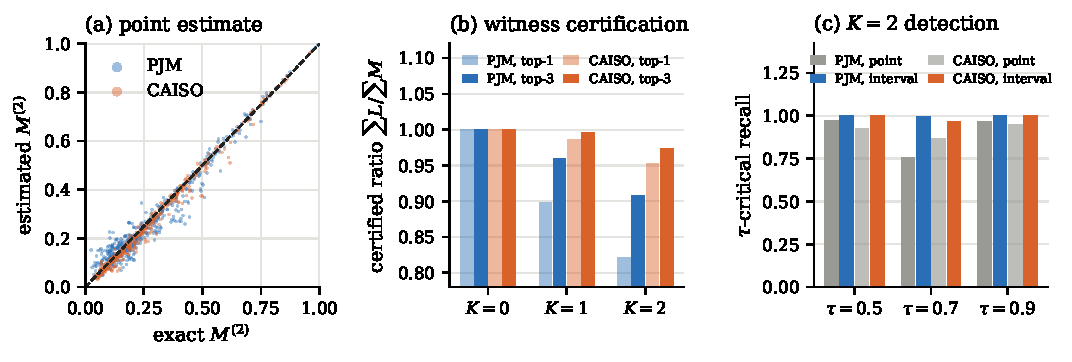
\includegraphics[width=\textwidth]{fig4_m_interval.pdf}
\caption{From point estimate to certified interval. (a) estimated versus exact $M^{(2)}$;
(b) certifying the top-three candidate witnesses instead of only the best one raises the
certified lower bound; (c) the interval-based conservative rule removes the recall deficit
of the point estimate.}
\label{fig:mint}
\end{figure}
Used as a decision rule, the interval removes the recall problem. Flagging $i$ as critical
whenever some background satisfies $\hat V(T)-\delta_\alpha \le \tau <
\hat V(T\cup\{i\})+\delta_\alpha$ raises recall at $K=2$, $\tau=0.7$ from $0.754$ to $0.994$
(PJM) and from $0.866$ to $0.967$ (CAISO), at the cost of precision falling to $0.870$ and
$0.826$. For a release audit this is the correct direction: false alarms are resolved by
retraining the flagged candidate, whereas misses are not resolved at all. One caveat is
recorded: at $\tau=0.9$ the global quantile $\delta_\alpha$ is too wide relative to the narrow
band of $V$ values near one, and precision falls to $0.420$ (PJM) and $0.657$ (CAISO);
a stratified $\delta$ would be needed if $\tau=0.9$ were the operating point.

\subsection{RQ-A5: efficiency, and when amortization is \emph{not} needed}
Table~\ref{tab:cost} gives measured costs on a single GPU. The result that matters most is
not the speedup but its scope: \textbf{at 41 fields the complete exact $K\le 2$ audit takes
about eleven minutes with batched dedicated retraining}, so amortization is not required to
make this audit feasible. The break-even query count against batched retraining is 2{,}816
(PJM) and 3{,}082 (CAISO) for the three-seed main estimator, and 495 and 562 for the
single-seed variant, which trades roughly $0.004$ of $V$ MAE for a $12\times$ cheaper query
(Table~\ref{tab:ablation}).

\begin{table}[t]
\centering
\caption{Measured wall-clock cost on PJM, single GPU. ``Full $K{=}2$'' is 11{,}521 sets;
``Full $K{=}3$'' is 112{,}791 sets. Amortized columns include backbone pre-learning
(27\,s per seed). The main estimator uses three seeds; the single-seed variant is the
cheaper configuration reported in Table~\ref{tab:ablation} as $\phi$ ridge.}
\label{tab:cost}
\small
\begin{tabular}{lrrrr}
\toprule
Workload & Sequential & Batched & Amortized & Amortized \\
         & retraining & retraining & (3 seeds, main) & (1 seed) \\
\midrule
Per query           & 21.8\,s & 56.6\,ms & 28.0\,ms & 2.4\,ms \\
$10^3$ queries      & 6.1\,h  & 1.6\,min & 1.8\,min & 0.5\,min \\
$10^5$ queries      & 606\,h  & 94\,min  & 48\,min  & 4.4\,min \\
Full $K{=}2$        & 70\,h   & \textbf{10.9\,min} & 6.7\,min & \textbf{0.9\,min} \\
Full $K{=}3$        & 683\,h  & 106\,min & 54\,min  & 4.9\,min \\
\midrule
Break-even vs.\ batched & --- & --- & 2{,}816 queries & 495 queries \\
\bottomrule
\end{tabular}
\end{table}

\begin{figure}[t]
\centering
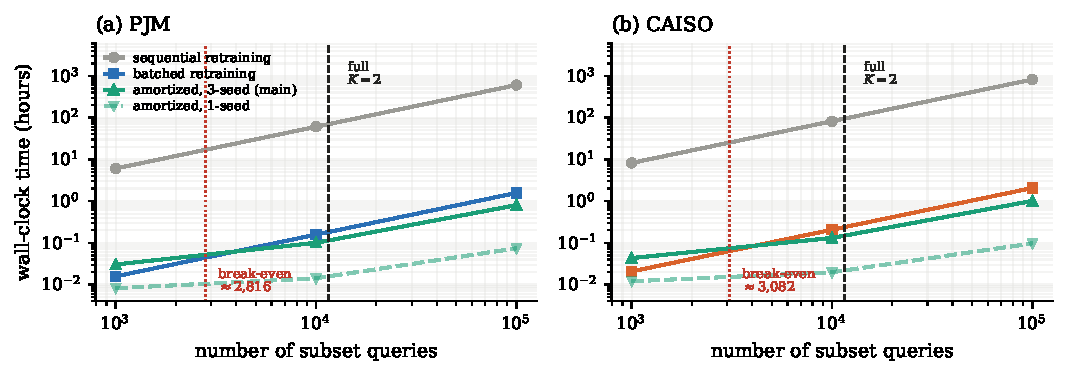
\includegraphics[width=\textwidth]{fig8_efficiency.pdf}
\caption{Cost of an audit as a function of the number of subset queries. The dashed vertical
line marks the complete $K=2$ sweep, which lies below the break-even point of the main
estimator: at 41 fields, batched dedicated retraining is the cheaper way to obtain the exact
table.}
\label{fig:eff}
\end{figure}
Amortization becomes material in the regimes the audit workloads actually generate: a full
$K=3$ sweep ($10^5$ queries), larger field spaces (extrapolating by set count, a complete
$K=2$ audit at $p=100$ comprises 166{,}750 sets, needing about 2.6\,h of batched retraining
versus 1.3\,h for the three-seed estimator and 7\,min for the single-seed variant),
dangerous-context search over large backgrounds, and repeated recomputation when the
baseline $B$, the data snapshot or the target changes. We state this scope explicitly rather
than presenting amortization as the only feasible route.

%===============================================================================
\section{Part B: Is $M$ the Right Field-Level Security Quantity?}\label{sec:exp-b}
%===============================================================================

\subsection{RQ-B1: what single-field and attribution methods miss}
Table~\ref{tab:detect} evaluates how well each score ranks fields by $\tau$-criticality,
using the exact $K=2$ ground truth as the label.

\begin{table}[t]
\centering
\caption{PR-AUC for detecting $\tau$-critical fields ($K=2$). Exact $M^{(2)}$ is an oracle
reference, not a deployable score.}
\label{tab:detect}
\small
\begin{tabular}{lrrrrrr}
\toprule
& \multicolumn{3}{c}{PJM} & \multicolumn{3}{c}{CAISO} \\
\cmidrule(lr){2-4}\cmidrule(lr){5-7}
Score & $\tau{=}0.5$ & $\tau{=}0.7$ & $\tau{=}0.9$ & $\tau{=}0.5$ & $\tau{=}0.7$ & $\tau{=}0.9$ \\
\midrule
Permutation importance (full model) & 0.779 & 0.675 & 0.165 & 0.798 & 0.460 & 0.181 \\
SAGE (full model)                   & 0.816 & 0.730 & 0.283 & 0.832 & 0.594 & 0.307 \\
Pearson $|r|$                       & 0.881 & 0.826 & 0.459 & 0.897 & 0.729 & 0.466 \\
Spearman $|\rho|$                   & 0.895 & 0.829 & 0.459 & 0.895 & 0.747 & 0.422 \\
Normalized mutual information       & 0.925 & 0.822 & 0.438 & 0.924 & 0.769 & 0.363 \\
Single-field $M^{(0)}$ (exact)      & 0.907 & 0.877 & 0.480 & 0.916 & 0.764 & 0.454 \\
Estimated $M^{(1)}$                 & \textbf{0.939} & \textbf{0.888} & \textbf{0.601} & 0.941 & 0.823 & 0.532 \\
Estimated $M^{(2)}$                 & 0.939 & 0.877 & 0.573 & \textbf{0.944} & \textbf{0.829} & \textbf{0.549} \\
\midrule
\emph{Exact $M^{(2)}$ (oracle)}     & 0.924 & 0.885 & 0.566 & 0.946 & 0.831 & 0.549 \\
\bottomrule
\end{tabular}
\end{table}

Full-model attribution is clearly unsuited to this task: SAGE reaches only 0.594 on CAISO at
$\tau=0.7$, below even Pearson correlation. The reason is structural rather than
statistical. These methods measure \emph{model reliance}---what one fitted model happens to
use---whereas disclosure risk is \emph{potential inference capability} over all attackers.
When several fields carry substitutable information, the fitted model commits to one and the
attribution assigns the others near-zero importance, even though each alone supports the
inference.

We also report an unfavorable result plainly. Exact single-field capability $M^{(0)}$ is a
strong ranking baseline: at PJM $\tau=0.7$ it reaches $0.877$ against $0.888$ for estimated
$M^{(1)}$, a gap of $0.011$. \emph{On the ranking task, $M$ is close to the best
single-field baseline.} The advantage of $M$ is not ranking; it is decision-making, which
the next subsection isolates. Restricting the evaluation to fields that are critical only in
combination ($K=2$ critical but $K=0$ safe) widens the gap slightly but does not change this
conclusion.

\subsection{RQ-B2/B3: escalation profiles and witnesses}
Averaged over 41 fields and 12 targets, mean $M$ rises from $0.144$ ($K{=}0$) to $0.242$
($K{=}1$) to $0.287$ ($K{=}2$) in PJM, and from $0.182$ to $0.255$ to $0.282$ in CAISO. Most
of the escalation therefore occurs at the \emph{first} background field, consistent with
Proposition~\ref{prop:k1}: a single super-additive partner is usually enough.

\begin{figure}[t]
\centering
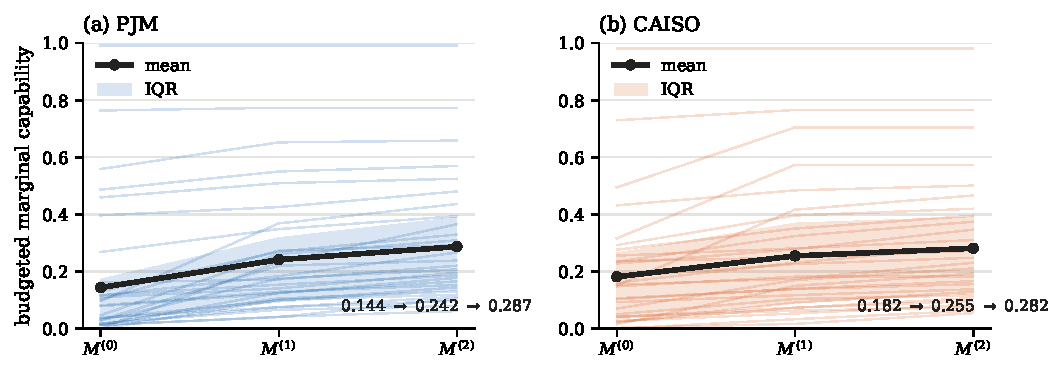
\includegraphics[width=\textwidth]{fig5_escalation.pdf}
\caption{Inference escalation profiles $M^{(0)}\to M^{(1)}\to M^{(2)}$ under the official
attacker family. Thin lines are individual (field, target) pairs; the shaded band is the
interquartile range. Most escalation occurs at the first background field.}
\label{fig:escal}
\end{figure}
The main text stops at $K=2$. A $K=3$ table exists but only under a weaker single-attacker
family, and the discrepancy between that family and the official one is \emph{larger than the
increment it would illustrate}: at $K=2$ the attacker-family gap is $0.0266$ (PJM) and
$0.0153$ (CAISO), while the $K{=}2 \to K{=}3$ increment within the weaker family is $0.0213$
and $0.0102$. Reporting them side by side would be misleading, so $K=3$ appears only in
\ref{app:k3}. The same comparison independently supports stopping at $K=2$: within a fixed
family, $M^{(2)}/M^{(3)} = 0.924$ (PJM) and $0.963$ (CAISO), so additional budget buys less
than switching to a stronger attacker.

Witnesses make a risk statement auditable: each flagged field comes with a concrete
background whose effect can be verified by retraining. We caution against over-reading them.
Under an independent discovery/audit split, the \emph{identity} of the witness reproduces
only 12--37\% of the time at $K\ge1$, while the field's risk level and $\tau$-critical status
reproduce at 0.78--1.00. A witness should therefore be presented as \emph{one verifiable
example} of a dangerous background, not as the unique dangerous combination.

\subsection{RQ-B4: risk is relative to what is already public}
Taking $B$ to be PJM's two publicly released load forecasts changes the picture
qualitatively. For \texttt{total\_gen} and \texttt{metered\_load}, $\Vy(B)$ is already
$0.974$ and $0.991$: the baseline alone leaks the target, and grading individual fields for
these targets is meaningless. For other targets the maximum $M^{(2)}$ drops sharply---for
\texttt{total\_lmp\_da} from $0.983$ to $0.406$---while reserve-type targets are almost
unaffected. The Kendall correlation between field rankings with and without $B$ ranges from
$0.47$ to $0.87$. Disclosure risk is thus a property of a field \emph{relative to the current
public baseline}, not an intrinsic attribute, which is why $B$ is explicit in
Definition~\ref{def:mk}.

\subsection{RQ-B5: release audit}\label{sec:release}
This is the decision-level comparison. For a representative target per market
(\texttt{total\_gen} for PJM, \texttt{actual\_load} for CAISO) we draw 2{,}000 random
size-three candidate release sets and apply six rules at $\tau=0.7$
(Table~\ref{tab:release}). A set is \emph{unsafe} if the retrained attacker family exceeds
$\tau$ on it.

\begin{table}[t]
\centering
\caption{Release audit, 2{,}000 random size-three sets, $\tau=0.7$. Dangerous release is the
fraction of unsafe sets that the rule accepts.}
\label{tab:release}
\small
\begin{tabular}{lrrrr}
\toprule
& \multicolumn{2}{c}{PJM} & \multicolumn{2}{c}{CAISO} \\
\cmidrule(lr){2-3}\cmidrule(lr){4-5}
Rule & Dangerous rel. & False rej. & Dangerous rel. & False rej. \\
\midrule
Single-field capability $\le\tau$            & 19.1\% & 0.0\%  & 56.4\% & 0.0\% \\
Correlation $\le 0.5$                        & 2.1\%  & 37.9\% & 3.2\%  & 22.6\% \\
Direct estimate $\hat V(A)\le\tau$           & 6.6\%  & 0.0\%  & 2.6\%  & 0.1\% \\
\textbf{Staged budget $U^{(2)}(A)\le\tau$}   & \textbf{0.0\%} & 49.6\% & \textbf{0.0\%} & 32.8\% \\
Additive budget $\sum \hat M \le\tau$        & 0.0\%  & 89.4\% & 0.0\%  & 69.4\% \\
Additive budget $\sum M \le\tau$ (exact)     & 0.0\%  & 86.3\% & 0.0\%  & 74.0\% \\
\bottomrule
\end{tabular}
\end{table}

\begin{figure}[t]
\centering
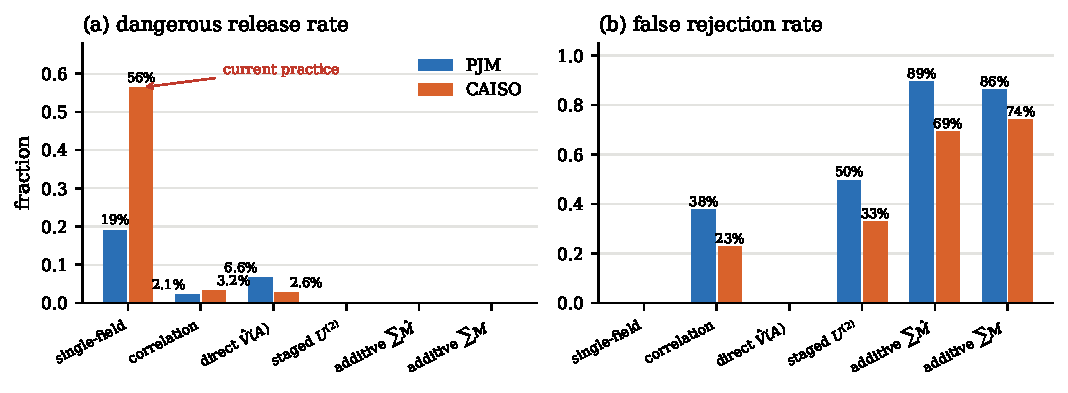
\includegraphics[width=\textwidth]{fig7_release_audit.pdf}
\caption{Release audit over 2{,}000 random size-three sets at $\tau=0.7$. The single-field
rule never rejects a safe set but accepts a large share of unsafe ones; the staged budget
accepts none at a rejection rate below one half.}
\label{fig:release}
\end{figure}
The single-field rule---current practice---accepts 19.1\% of unsafe PJM sets and 56.4\% of
unsafe CAISO sets while never rejecting a safe one. It is not conservative; it is blind in
one direction. The additive budget of Theorem~\ref{thm:super}(a) eliminates dangerous
releases but rejects 69--89\% of safe sets, which no operator would deploy. The staged budget
$U^{(2)}$ of Theorem~\ref{thm:super}(b) is the only rule achieving zero dangerous release at
a rejection rate below one half. The direct amortized estimate has almost no false
rejections but still admits 2.6--6.6\% dangerous releases, making it a good \emph{pre-filter}
and a poor final gate. A practical deployment combines them: screen with $U^{(2)}$, and
re-examine rejected sets with the direct estimate plus certified retraining.

The corresponding field grading is summarized in Table~\ref{tab:grading}. The last column is
the paper's opening claim, now measured.

\begin{table}[t]
\centering
\caption{Field grading at $\tau=0.7$, $K=2$, representative target per market.}
\label{tab:grading}
\small
\begin{tabular}{lrrrr}
\toprule
Market & Fields & $K{=}2$ critical & Critical alone & \textbf{Safe alone, critical with $\le 2$} \\
\midrule
PJM   & 41 & 40 & 5 & \textbf{35} \\
CAISO & 41 & 41 & 3 & \textbf{38} \\
\bottomrule
\end{tabular}
\end{table}

\subsection{RQ-B6: how much auxiliary data does the adversary need?}\label{sec:exp-naux}
All results so far assume the adversary trains on the same amount of data as the auditor.
We relax this by giving the adversary a nested $10\%$, $25\%$, $50\%$ or $100\%$ of the
auxiliary labels, with training \emph{and} model selection confined to that subset.

\paragraph{Inferability degrades gracefully.}
At $10\%$ (459 PJM / 610 CAISO records) the mean $\Vy$ over size-three sets retains $80.7\%$
and $90.2\%$ of its full-data value. Data scarcity is not an effective defense.

\paragraph{Auditing with a weak attacker is unsafe.}
If the auditor evaluates and releases using a $10\%$ attacker while the real adversary has
full data, $25.6\%$ (PJM, $\tau{=}0.5$) and $13.2\%$ (CAISO) of genuinely exploitable sets
are released; $\tau$-critical recall falls to $0.565$ (PJM, $\tau{=}0.7$). Precision stays
at $0.89$--$1.00$, so the error is purely one-directional. This is the empirical argument for
taking the maximum over an attacker family rather than fixing one attacker.

\paragraph{$\Mik$ is inflated, not deflated, under weak attackers.}
Counterintuitively, although $\Vy$ is uniformly underestimated, $M^{(1)}$ and $M^{(2)}$
\emph{exceed} their full-data values by 5--12\% (Table~\ref{tab:naux}), while $M^{(0)}$
remains monotone. The mechanism is that $\Mik$ is a \emph{maximum} statistic: noisy marginals
combined with a maximum over backgrounds systematically select positive noise. Decomposing
$M_{\mathrm{frac}}-M_{\mathrm{full}} = \underbrace{[M_{\mathrm{frac}}-\Delta_{\mathrm{frac}}
(T_{\mathrm{full}})]}_{\text{selection gain}} - \underbrace{[M_{\mathrm{full}}-
\Delta_{\mathrm{frac}}(T_{\mathrm{full}})]}_{\text{genuine underestimation}}$ confirms this:
the selection gain grows with the number of candidate backgrounds---identically zero at
$K{=}0$ (one candidate), $0.021$ at $K{=}1$ (41 candidates) and $0.081$ at $K{=}2$ (821
candidates) for PJM at $10\%$. Consistently, the witness selected at $10\%$ agrees with the
full-data witness only $11.6\%$ of the time and retains only $77.4\%$ of its effect.

\begin{table}[t]
\centering
\caption{Attacker-capability sensitivity. $M$ values are ratios to the full-data value;
the selection-gain decomposition is at $K=2$.}
\label{tab:naux}
\small
\begin{tabular}{llrrrrr}
\toprule
Market & Aux.\ labels & $\Vy$ ratio & $M^{(0)}$ & $M^{(1)}$ & $M^{(2)}$ & Sel.\ gain ($K{=}2$) \\
\midrule
\multirow{4}{*}{PJM}
 & 10\% (459)   & 0.807 & 0.855 & 0.923 & \textbf{1.077} & 0.081 \\
 & 25\% (1147)  & 0.907 & 0.928 & 0.998 & \textbf{1.124} & 0.060 \\
 & 50\% (2294)  & 0.958 & 0.974 & 0.984 & 1.023 & 0.025 \\
 & 100\% (4589) & 1.000 & 1.000 & 1.000 & 1.000 & 0.000 \\
\midrule
\multirow{4}{*}{CAISO}
 & 10\% (610)   & 0.902 & 0.927 & 0.979 & \textbf{1.053} & 0.041 \\
 & 25\% (1526)  & 0.963 & 0.965 & 1.013 & \textbf{1.046} & 0.021 \\
 & 50\% (3052)  & 0.989 & 0.987 & 1.009 & 1.018 & 0.010 \\
 & 100\% (6105) & 1.000 & 1.000 & 1.000 & 1.000 & 0.000 \\
\bottomrule
\end{tabular}
\end{table}

\begin{figure}[t]
\centering
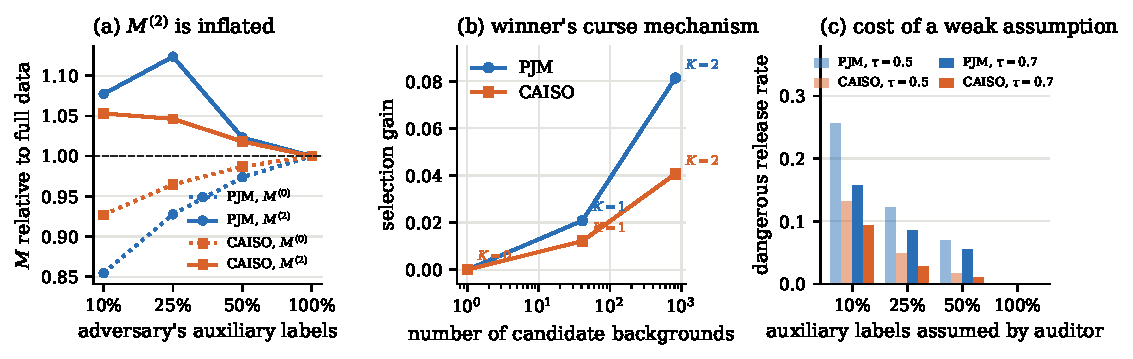
\includegraphics[width=\textwidth]{fig9_attacker_capability.pdf}
\caption{Attacker-capability sensitivity. (a) $M^{(2)}$ exceeds its full-data value when the
adversary is weak, while $M^{(0)}$ does not; (b) the selection gain grows with the number of
candidate backgrounds, identifying a maximum-statistic bias; (c) auditing under a weak
attacker assumption releases sets that a full-data attacker can exploit.}
\label{fig:naux}
\end{figure}
This has a direct methodological consequence: \textbf{point estimates of $\Mik$ must not be
compared across sample sizes or attacker strengths}, and any reported $\Mik$ should be
accompanied by the certified lower bound of Section~\ref{sec:interval}. Note that this is a
\emph{second, mechanically distinct} reason for the interval---Section~\ref{sec:interval}
addresses estimator error, whereas the selection bias here would arise even with a perfect
estimator applied to a weaker attacker.

%===============================================================================
\section{Discussion}\label{sec:discussion}
%===============================================================================

\paragraph{When is amortization worth it?}
Not at $p=41$ with $K\le 2$, where exact batched retraining takes eleven minutes. It becomes
worthwhile at $10^5$-query workloads, larger field spaces, interactive auditing, and whenever
the baseline, data snapshot or target changes and the whole table must be recomputed. We
prefer to state this boundary rather than motivate the method with an infeasibility that does
not hold at the scale we can verify.

\paragraph{Ranking versus deciding.}
Exact single-field capability ranks fields nearly as well as $M$ (Table~\ref{tab:detect}).
The value of $M$ appears at the decision layer, where a rule must accept or reject a
concrete set (Table~\ref{tab:release}). This distinction should be kept explicit: a reader
comparing only PR-AUC would reasonably conclude that the simpler score suffices.

\paragraph{Two biases, one remedy.}
The estimator underestimates $M$ for some fields; a weak attacker inflates it for many.
The mechanisms are unrelated but the remedy is the same---report $[L,U]$, with $L$ certified
by retraining the proposed witnesses. This is also why we retain dedicated retraining in the
pipeline rather than replacing it: the amortized model generates candidates, and retraining
certifies them.

\paragraph{Limitations.}
\emph{(i)} We evaluate under random splits and do not assess temporal extrapolation;
distribution drift may change the numerical values of $M$, although the audit framework
itself is independent of how the data is split. \emph{(ii)} Witness identity does not
reproduce across independent data splits, so witnesses are examples, not unique certificates.
\emph{(iii)} The upper bound's coverage relies on an exchangeability assumption across
held-out fields and is not a finite-sample guarantee. \emph{(iv)} For backgrounds of size
four and above we have lower bounds only. \emph{(v)} The threshold $\tau$ is exogenous; we
report three values and their sensitivity rather than advocating one. \emph{(vi)} The
interval's conservative decision rule loses precision at $\tau=0.9$. \emph{(vii)} The
attacker family, though maximized over three members, excludes XGBoost and LightGBM variants
and random forests; a stronger family would raise ground truth and, by the logic of
Section~\ref{sec:exp-naux}, could only increase the measured combination risk.
\emph{(viii)} The sensitivity study of Section~\ref{sec:exp-naux} uses a single attacker and
one seed per fraction.

%===============================================================================
\section{Conclusion}\label{sec:conclusion}
%===============================================================================

Screening power-market fields one at a time is not a conservative approximation of a
combination-aware audit; it fails in the unsafe direction. Formalizing the audit as
estimation of set-level inferability, and converting it into a field-level quantity through
the budgeted marginal inference capability $\Mik$, makes the gap measurable: on two markets,
35 of 41 and 38 of 41 fields are safe alone and critical with at most two background fields,
and a single-field release rule admits 19.1\% and 56.4\% of genuinely unsafe sets. The
truncated super-efficiency bound turns the field-level table into a staged release rule that
admits none of them while rejecting fewer than half of the safe sets. Two independent biases
in the point estimate---estimator error and the selection bias of a maximum statistic under
weak attackers---are both handled by reporting a certified lower bound with a calibrated
upper bound. Extending the evidence to field spaces of a hundred or more, and to a third
market, is the natural next step.

%===============================================================================
\appendix
\section{Remaining proofs}\label{app:proofs}
%===============================================================================

\begin{proposition}[Ladder, monotonicity in the candidate set, duplication invariance]
\label{prop:ladder}
\emph{(a)} $M^{(0)}_{i\to y}\le M^{(1)}_{i\to y}\le\cdots\le M^{(|H|-1)}_{i\to y}$;
\emph{(b)} enlarging the candidate set from $H$ to $H'\supseteq H$ cannot decrease
$\Mik$; \emph{(c)} if $f'$ is a duplicate of $f$, i.e.\ $\Vy(B\cup T\cup\{f'\}) =
\Vy(B\cup T\cup\{f\}) = \Vy(B\cup T\cup\{f,f'\})$ for all $T$, then deleting $f'$ leaves
$\Mik$ unchanged for every $i \ne f,f'$.
\end{proposition}
\begin{proof}
(a) and (b) are maxima over larger feasible sets. (c) Let $T$ be a witness for $i$
containing $f'$. If $f\notin T$, replace $T$ by $(T\setminus\{f'\})\cup\{f\}$: same size,
same value. If $f\in T$, replace $T$ by $T\setminus\{f'\}$: smaller size, same value. Either
replacement stays within budget, so the maximum does not decrease after deleting $f'$; by (b)
it does not increase either.
\end{proof}

\begin{proposition}[Field-level bound on irreducible synergy]\label{prop:syn}
Define the irreducible gain of $S$ as
$\mathrm{syn}^{B}(S)=\Vy(B\cup S)-\max_{T\subsetneq S}\Vy(B\cup T)$. For $|S|\ge 2$,
$\mathrm{syn}^{B}(S)\le \min_{j\in S} M^{(|S|-1)}_{j\to y}$.
\end{proposition}
\begin{proof}
$\max_{T\subsetneq S}\Vy(B\cup T)\ge \Vy(B\cup S\setminus\{j\})$, hence
$\mathrm{syn}^{B}(S)\le \Delta_j(B\cup S\setminus\{j\})\le M^{(|S|-1)}_{j\to y}$.
\end{proof}

\begin{remark}
Proposition~\ref{prop:syn} fails if strength is measured by the Harsanyi
dividend~\cite{harsanyi1963dividend}: with $\Vy(\{i\})=0.5$ for $i=1,2,3$,
$\Vy(\{i,j\})=0.5$ and $\Vy(\{1,2,3\})=1.0$, the dividend of the triple is $1.0$ while
$M^{(2)}=0.5$. This is why we define strength as the irreducible gain.
\end{remark}

\begin{remark}[Escalation and submodularity]
Let $\Gamma^{(K)}_i := \Mik - M^{(0)}_{i\to y}$. Then $\Gamma^{(K)}_i=0$ if and only if
$\Delta_i(B\cup T)\le\Delta_i(B)$ for all $|T|\le K$. This is strictly weaker than
submodularity: submodularity implies no escalation, but not conversely. A three-field
monotone counterexample is $\Vy(\{1\})=0.8$, $\Vy(\{2\})=0.6$, $\Vy(\{3\})=0.8$, all pairs
$0.8$, and $\Vy(\{1,2,3\})=1.0$: every field has $M^{(2)}=a$, yet
$\Delta_1(\{3\})=0<\Delta_1(\{2,3\})=0.2$. Hence ``escalation $\iff$ synergy'' is not a
valid reading.
\end{remark}

\section{$K=3$ under the reduced attacker family}\label{app:k3}
Exhaustive size-four retraining is available only for the multi-target network. Mean $M$
under that family is $0.1346/0.2262/0.2608/0.2821$ for PJM at $K=0,1,2,3$ and
$0.1766/0.2455/0.2664/0.2766$ for CAISO. The corresponding values under the official
three-attacker family at $K\le 2$ are $0.1443/0.2417/0.2873$ (PJM) and
$0.1820/0.2550/0.2817$ (CAISO). Since the family gap at $K=2$ ($0.0266$ / $0.0153$) exceeds
the $K{=}2\to K{=}3$ increment within the weaker family ($0.0213$ / $0.0102$), these columns
must not be read as a continuation of the main-text escalation curve.

\bibliographystyle{elsarticle-num}
\bibliography{ref}

\end{document}
